 %%
%%
\documentclass[12pt]{book}
\usepackage{amsfonts}
\usepackage{amsmath}
\usepackage{amsthm}
\usepackage{amssymb}
\usepackage{graphicx}
\usepackage{hyperref}
\setlength{\textheight}{10in}
\setlength{\textwidth}{7.4in}
\setlength{\topmargin}{-0.75in}
\setlength{\oddsidemargin}{-0.5in}
\setlength{\evensidemargin}{-0.5in}
\setlength{\parskip}{0.15in}
\setlength{\parindent}{0in}

\begin{document}


\vspace{-1.0in}\begin{center}
\Large{MHF4U :  Advanced Functions }

\Large{Assignment \#3}


\end{center}

%\medskip

\vspace{0.015in}\hrulefill\ 

\textbf{Reference Declaration} %  Fill in your Reference Declarations in this section before your submit your assignment.
Complete the Reference Declaration section below in order for your assigment to be graded.

If you used any references beyond the course text and lectures (such as other texts, discussions with peers or online resources), indicate this information in the space below.  If you did not use any aids, state this in the space provided. 

Be sure to cite appropriate theorems throughout your work. You may use shorthand for well-known theorems like the FT (Factor Theorem), RRT (Rational Root Theorem), etc. 

Note: Your submitted work must be \textbf{your original work}. 

Family Name: Wong\\%Family Name Here
First Name: Max%First Name Here

Declared References: 

% Type your references here.
% You can use as many lines as required.

\vspace{0.015in}\hrulefill\ 

\newpage

%%%%%%%%%%%% PROBLEMS START HERE

\begin{enumerate}

%% PROBLEM 1
\item Prove the identity $\sin(x)\cos(x)=1-\dfrac{\sin^2(x)}{1+\cot(x)}-\dfrac{\cos^2(x)}{1+\tan(x)}$. Remember to use proper form for proving trigonometric identities by indicating the identities you are using.

\vspace{-0.4cm}
\textbf{Solution to Question 1:}
We can prove the identity by getting one side of the equal sign to be equivalent to the other side.
\vspace{-3cm}

\begin{proof}
\addtolength{\jot}{1em}
\begin{align*}
    RHS &= 1-\dfrac{\sin^2(x)}{1+\cot(x)}-\dfrac{\cos^2(x)}{1+\tan(x)} && \text{RHS: Right Hand Side} \\
    &= 1-\dfrac{\sin^2(x)}{1+\dfrac{1}{tan(x)}}-\dfrac{\cos^2(x)}{1+\tan(x)} && cot(x) = \dfrac{1}{tan(x)} \\
    &= 1-\dfrac{\sin^2(x)}{1+\dfrac{1}{\dfrac{\sin(x)}{\cos(x)}}}-\dfrac{\cos^2(x)}{1+\dfrac{\sin(x)}{\cos(x)}} && tan(x) = \dfrac{\sin(x)}{\cos(x)} \\
    &= 1-\dfrac{\sin^2(x)}{1+\dfrac{\cos(x)}{\sin(x)}}-\dfrac{\cos^2(x)}{1+\dfrac{\sin(x)}{\cos(x)}} && \text{Simplify} \\
    &= 1-\dfrac{\sin^2(x)}{\dfrac{\sin(x)}{\sin(x)} +\dfrac{\cos(x)}{\sin(x)}}-\dfrac{\cos^2(x)}{1+\dfrac{\sin(x)}{\cos(x)}} && 1 = \dfrac{\sin(x)}{\sin(x)} \\
    &= 1-\dfrac{\sin^2(x)}{\dfrac{\sin(x)}{\sin(x)} +\dfrac{\cos(x)}{\sin(x)}}-\dfrac{\cos^2(x)}{\dfrac{\cos(x)}{\cos(x)}+\dfrac{\sin(x)}{\cos(x)}} && 1 = \dfrac{\cos(x)}{\cos(x)} \\
    &= 1-\dfrac{\sin^2(x)}{\dfrac{\sin(x) + \cos(x)}{\sin(x)}}-\dfrac{\cos^2(x)}{\dfrac{\sin(x) + \cos(x)}{\cos(x)}} && \text{Simplfy} \\
    &= 1-\sin^2(x) \div \dfrac{\sin(x) + \cos(x)}{\sin(x)} - \cos^2(x) \div \dfrac{\sin(x) + \cos(x)}{\cos(x)} && \dfrac{a}{b} = a \div b \\
    &= 1-\sin^2(x) \times \dfrac{\sin(x)}{\sin(x) + \cos(x)} - \cos^2(x) \times \dfrac{\cos(x)}{\sin(x) + \cos(x)} && \text{Convert } \div \text{ to } \times \text{ with reciprocal} \\
    &= 1-\dfrac{\sin^3(x)}{\sin(x) + \cos(x)} - \dfrac{\cos^3(x)}{\sin(x) + \cos(x)} && \text{Simplify} \\
\end{align*}

\addtolength{\jot}{1em}
\begin{align*}
    RHS &= \dfrac{\sin(x)+\cos(x)}{\sin(x)+\cos(x)}-\dfrac{\sin^3(x)}{\sin(x) + \cos(x)} - \dfrac{\cos^3(x)}{\sin(x) + \cos(x)} && 1 = \dfrac{\sin(x)+\cos(x)}{\sin(x)+\cos(x)} \\
    &= \dfrac{\sin(x)+\cos(x) - \sin^3(x) - \cos^3(x)}{\sin(x)+\cos(x)} && \text{Simplfy} \\
    &= \dfrac{\sin(x)+\cos(x) -(\sin(x))(\sin^2(x))  - (\cos(x))(\cos^2(x))}{\sin(x)+\cos(x)} && a^3 = a\times a^2\\
    &= \dfrac{\sin(x)+\cos(x) -(\sin(x))(1 - \cos^2(x))  - (\cos(x))(\cos^2(x))}{\sin(x)+\cos(x)} && \sin^2(x) = 1 - \cos^2(x) \\
    &= \dfrac{\sin(x)+\cos(x) -(\sin(x))(1 - \cos^2(x))  - (\cos(x))(1 - \sin^2(x))}{\sin(x)+\cos(x)} && \cos^2(x) = 1 - \sin^2(x) \\
    &= \dfrac{\sin(x)+\cos(x) -(\sin(x) - \cos^2(x)\sin(x))  - (\cos(x) - \sin^2(x)\cos(x))}{\sin(x)+\cos(x)} && \text{Expand} \\
    &= \dfrac{\sin(x)+\cos(x) - \sin(x) + \cos^2(x)\sin(x)  - \cos(x) + \sin^2(x)\cos(x)}{\sin(x)+\cos(x)} && \text{Break brackets}\\
    &= \dfrac{\cos^2(x)\sin(x) + \sin^2(x)\cos(x)}{\sin(x)+\cos(x)} && \text{Simplify}\\
    &= \dfrac{(\sin(x)\cos(x))(\sin(x) + \cos(x))}{\sin(x)+\cos(x)} && \text{Factor } \sin(x)\cos(x)\\
    &= \sin(x)\cos(x) && \text{Simplify}\\
    &= RHS \qedhere\\
\end{align*}
\end{proof}

\vspace{-1cm}
$$\therefore \sin(x)\cos(x)=1-\dfrac{\sin^2(x)}{1+\cot(x)}-\dfrac{\cos^2(x)}{1+\tan(x)}$$

\newpage

%% PROBLEM 2
\item Determine equivalent expressions for both of $\sin(4x)$ and $\cos(4x)$ entirely in terms of $x$. You do not need to justify your steps.

\textbf{Expand and simplify sin(4x) using indentities:}
\addtolength{\jot}{1em}
\begin{align*}
    \sin(4x) &= ? \\
    \sin(4x) &= \sin(2x+2x) && 2x+2x=4x \\
    &= 2\sin(2x)\cos(2x) && \text{Double Angle Identity for sine where angle is 4x}\\
    &= 2(2\sin(x)\cos(x))\cos(2x) && \text{Double Angle Identity for sine where angle is 2x}\\
    &= 2(2\sin(x)\cos(x))(\cos^2(x)-\sin^2(x)) && \text{Double Angle Identity for cosine where angle is 2x}\\
    &= 4\sin(x)\cos(x)(\cos^2(x)-\sin^2(x)) && \text{Expand}\\
    \therefore \sin(4x) &= \boxed{4\sin(x)\cos^3(x)-4\sin^3(x)\cos(x)}\\
\end{align*}

\textbf{Expand and simplify cos(4x) using indentities:}
\begin{align*}
    \cos(4x) &= ? \\
    \cos(4x) &= \cos(2x+2x) && 2x+2x=4x \\
    &= \cos^2(2x) - \sin^2(2x) && \text{Double Angle Identity for cosine where angle is 4x}\\
    &= (\cos^2(x) - \sin^2(x))^2 - \sin^2(2x) && \text{Double Angle Identity for cosine where angle is 2x}\\
    &= (\cos^2(x) - \sin^2(x))^2 - (2\sin(x)\cos(x))^2 && \text{Double Angle Identity for sine where angle is 2x}\\
    &= \cos^4(x) - 2\sin(x)^2\cos(x)^2 + \sin^2(x))^4 - 4\sin(x)^2\cos(x)^2 && \text{Apply exponents}\\
    \therefore \cos(4x) &= \boxed{\cos^4(x) + \sin^2(x))^4 - 6\sin(x)^2\cos(x)^2} && \text{Simplify}\\
\end{align*}

\newpage

%% PROBLEM 3
\item A circle is centered at the origin with a radius of 25. Inside this circle is an inscribed rectangle with its bottom edge on the x-axis and the two vertices on the opposite side on the circumference of the circle,. Represent the area, $A$, of the rectangle:

\begin{enumerate}
\item In terms of $x$, the distance between the y-axis and the right leg of the rectangle. 
\item In terms of $\theta$, where $\theta$ is an angle in standard position with its terminal arm on the upper right vertex of the rectangle.
\end{enumerate}

%%% You can omit the inclusion of these images from your own submission.

%\begin{figure}[h]
%\centering
%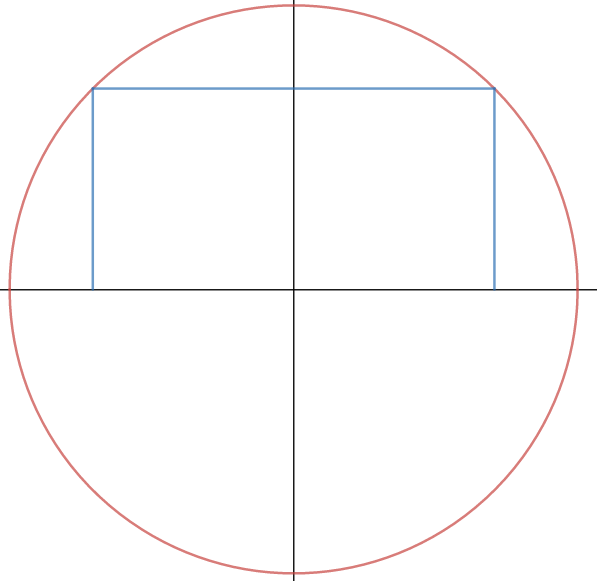
\includegraphics[scale=0.25]{Inscribed1.png}
%\caption{Diagram for part a}
%\end{figure}

%\begin{figure}[h]
%\centering
%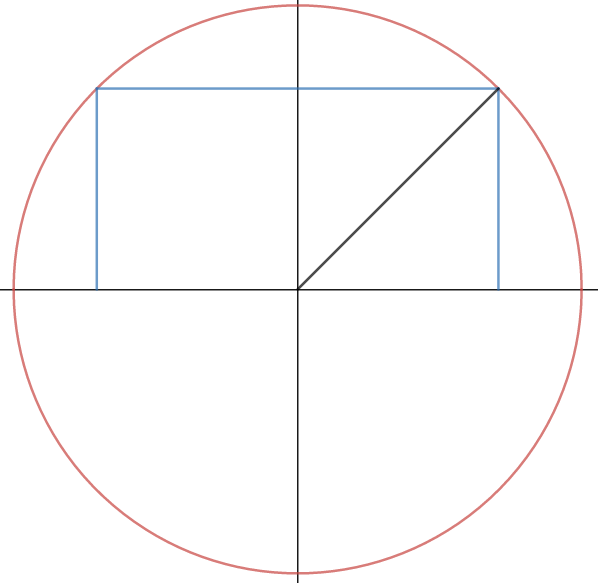
\includegraphics[scale=0.25]{Inscribed2.png}
%\caption{Diagram for part b}
%\end{figure}

\vspace{0.5cm}
\textbf{Solution for question 3 (a):}
\vspace{0.3cm}
First, let's get some labels. Take the inscribed rectangle and 
label the origin B, the top right corner A and the bottom corner C.
ABC form a right triangle. Label the appropriate sides 
with their corresponding angles.

%Diagram here
\begin{center}
    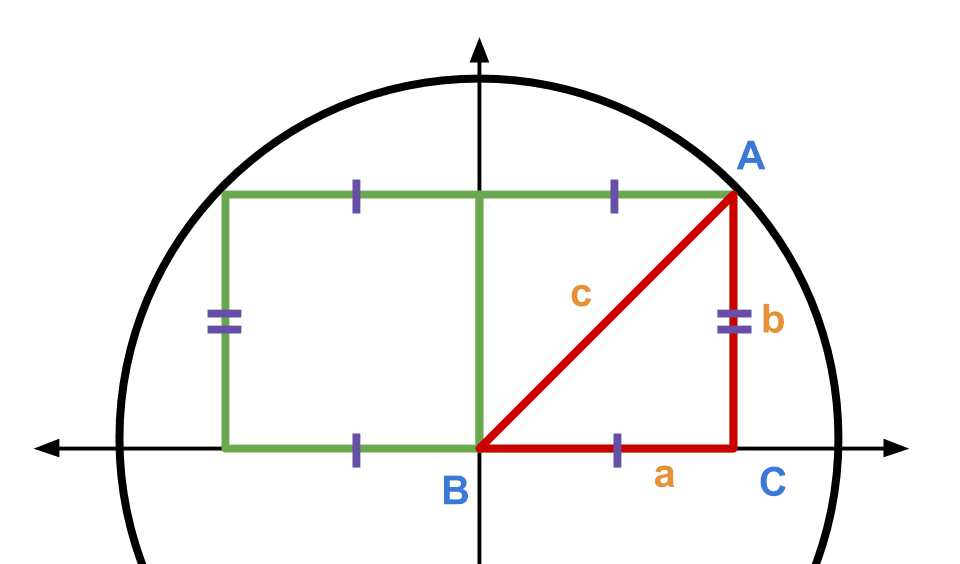
\includegraphics[scale = 0.25]{A3-3 Diagram.png}
\end{center}

\vspace{0.3cm}
We know that C or the radius is 25 units. We also know that (a) 
asks us to express the area with respect to "a" or the distance 
between the y-axis and the right leg of the rectangle.

From Pythagorean Theorum, we can also define b with respect to a and c:
\begin{align*}
    a^2 + b^2 &= c^2 \\
    b^2 &= c^2 - a^2 && \text{Subtract } a^2 \text{ from both sides}\\
    b &= \sqrt{c^2 - a^2} && \text{Square root } a^2 \text{ from both sides}\\
\end{align*}

\vspace{-0.5cm}
When we look at the diagram, we can see that the big rectangle is split in 
half by the y-axis. We can assume that both halfs are of the same dimensions 
and thus area because both halfs only touch the circle at 1 point and since 
they the circle is centered around the origin and both halfs share the same 
horizontal lines (and thus same height), using pythagorean theorem their 
x-distance from the origin must also be the same (same length/base).

\vspace{0.3cm}
If we solve the area of one half, we can multiply it by 2 to get the full area. 
The area of a rectangle is $base \times height, \therefore$ the area of the parent rectangle 
is $A = 2\times base \times height$ where A is the are, b is base and h is height. We know the base and height as a and b 
so let's substitute them in. 

\begin{align*}
    A &= 2bh \\
    A &= 2\times a \times b && \text{base = a, height = b} \\
    &= 2\times a \times \sqrt{c^2 - a^2} && b = \sqrt{c^2 - a^2} \\
    &= 2\times a \times \sqrt{25^2 - a^2} && \text{c = radius = 25} \\
    A &= 2\times a \times \sqrt{625 - a^2} && \text{Simplify} \\
\end{align*}

\vspace{-1cm}
$$\boxed{\therefore \text{The area of the rectangle in relation to a is } 2a\sqrt{625 - a^2}}$$

\vspace{0.5cm}
\textbf{Solution for question 3 (b):}

\vspace{0.3cm}
Taking (a)'s solution, we can biggy back on the previously done work. We know that 
Area is:

\begin{center}
    $2a\sqrt{625 - a^2}$ \textbf{(1)} 
\end{center}

\vspace{0.2cm}
If we can find the value of a in terms of $\theta$, 
we can substitute this value into (a)'s solution and determine the area.

\vspace{0.3cm}
Since B is the target angle, I will now refer the angle B as $\theta$. 
Let's try and define $\cos(\theta)$ by using the labeling system from (a). 
Consider the following:

$$\cos(\theta) = \frac{adj}{hyp} = \frac{a}{c} \text{\space \space \space (2)}$$

We want to isolate "a" within (2). If we multiply the whole equation by c, we can 
cancel out the denominator in $\frac{a}{c}$.

\begin{align*}
    \cos(\theta) &= \frac{a}{c} \\
    c \times \cos(\theta) &= \frac{a}{c} \times c && \text{Multiply all by c}\\
    c\cos(\theta) &= a && \text{Simplify}\\
    25\cos(\theta) &= a && \text{Since } c = 25\\
\end{align*}

\newpage

\begin{center}
    Now that we know the value of a, substitute this back into (1), the solution of (a):
\end{center}
\vspace{-0.5cm}

\begin{align*}
    A &= 2a\sqrt{625 - a^2} \\
    &= 2(25\cos(\theta))\sqrt{625 - (25\cos(\theta))^2} && a=25\cos(\theta)\\
    &= 50\cos(\theta)\sqrt{625 - 625\cos^2(\theta)} && \text{Simplify}\\
    &= 50\cos(\theta)\sqrt{625(1 - \cos^2(\theta))} && \text{Factor 625}\\
    &= 50\cos(\theta)\sqrt{625} \sqrt{1 - \cos^2(\theta)} && \sqrt{ab} = \sqrt{a}\sqrt{b}\\ %////////////////////////////TODO| Name Theorum
    &= 50\cos(\theta)25 \sqrt{1 - \cos^2(\theta)} && \text{Simplify} \\
    A &= 1250\cos(\theta)\sqrt{1 - \cos^2(\theta)} \\
\end{align*}

\vspace{-0.5cm}
$$\boxed{\therefore \text{ The area in relation to } \theta \text{ is } 1250\cos(\theta)\sqrt{1 - \cos^2(\theta)}}$$

\newpage


%% PROBLEM 4
\item Solve $2\sin^2(x) + \sin(2x) = 2$ $(x \in \mathbb{R})$. Be sure to effectively communicate the multiple solutions.

\textbf{To solve question 4, we need to factor the function:}

\begin{align*}
    2\sin^2(x) + \sin(2x) &= 2 \\
    2(1-\cos^2(x)) + \sin(2x) &= 2 && sin^2(x) = 1 - cos^2(x) \\
    2(1-\cos^2(x)) + 2\sin(x)\cos(x) &= 2 && \sin(2x) = 2\sin(x)\cos(x) \\
    2-2\cos^2(x) + 2\sin(x)\cos(x) &= 2 && \text{Expand}\\
    2 - 2 - 2\cos^2(x) + 2\sin(x)\cos(x) &= 0 && \text{Subtract 2 from both sides}\\
    - 2\cos^2(x) + 2\sin(x)\cos(x) &= 0 && \text{Simplify}\\
    - 2\cos(x)(\cos(x) - 2\sin(x)) &= 0 && \text{Factor } -2\cos(x)\\
\end{align*}

From this, we know that cos(x) is equal to 0 and sin(x). With this, we can solve for the value of x.

\vspace{0.3cm}
\underline{When cos(x) = 0}

\vspace{0.1cm}
$x = \boxed{\dfrac{\pi}{2}}$. Cosine is also positive in quadrant 4 meaning that there is a 
related accute angle in Q4:

$x = 2\pi - \dfrac{\pi}{2} = \boxed{\dfrac{3\pi}{2}}$

\vspace{0.3cm}
\underline{When cos(x) = sin(x)}
$\cos(x) = \sin(x)$ can also be expressed alternatively as $tan(x) = 1$ with the following procedure:

\begin{align*}
    \cos(x) &= \sin(x) \\
    \dfrac{\cos(x)}{\sin(x)} &= 1 && \text{Divide both sides by } \sin(x) \\
    \tan(x) &= 1 && \text{Quotient identity} \\ 
\end{align*}

We know that tan(x) = 1 when x is $\boxed{\dfrac{\pi}{4}}$. Since tangent is positive in 
quadrant 4, the related accute angle is in Q3. 

$x = \pi + \dfrac{\pi}{4} = \boxed{\dfrac{5\pi}{4}}$

\newpage

$$\therefore x = \dfrac{\pi}{4}, \dfrac{\pi}{2}, \dfrac{5\pi}{4} , \dfrac{3\pi}{2} \text{ if } x \in [0, 2\pi]$$

but the question states that $x \in \mathbb{R}$. We must create a pattern that extends 
infinitly. We know that this pattern repeats at every period or $2\pi$.

$$\boxed{\therefore x = \dfrac{\pi}{4} + 2\pi n, \dfrac{\pi}{2} + 2\pi n, \dfrac{5\pi}{4} + 2\pi n , \dfrac{3\pi}{2} + 2\pi n \text{ where } k \in \mathbb{Z}}$$

\vspace{0.1cm}


\newpage

%% PROBLEM 5
%\begin{minipage}{4in}
\item Go to the website of the \href{http://worldweather.wmo.int/}{World Meteorological Organization} and select a city from the map (right).
Once you select a city, click on Climatological Information which is a tab above the map. Locate and record the data for mean max. temperature and mean min. temperature into a table. Using the data, create models for the relationship between the day of the year and both the high and low mean respectively. Finally, test the accuracy of each model by using it to determine the temperature for a single day, each.
%\end{minipage}\hspace{0.2in}
%\begin{minipage}{1in}
%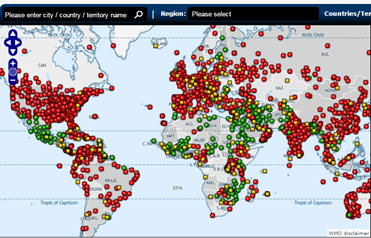
\includegraphics[scale=0.75]{WorldMap.png}
%\end{minipage}

\vspace{0.3cm}
\textbf{The process for solving question 5:}

\vspace{0.3cm}
From the data, we need to approximate key characteristics and values in order to form 
eventually form the function. We will perform this process for the mean max and mean 
min relationships seperately.

\vspace{0.3cm}
Note that I used July and January as my highest and lowest points (for amplitusde, axis) 
because this pairing overall gets the closest to the highest and lowest points. As a result 
the equation needs a horizontal shift by a month (30 days) to try and correct for the 7 month 
gap between Jan and July.

\vspace{0.3cm}
\underline{Mean Max}

\vspace{0.3cm}
\begin{tabular}{l|l}
    Period & 365 days \\
    Max & 23.1 \\
    Min & 2.7 \\
    Amplitude & =(Max+Min)/2\\
    Axis & \\

\end{tabular}

\underline{Mean Min}

\newpage


\end{enumerate}
\end{document} 
